\chapter{Evaluation}
\label{chap:evaluation}

Following chapter \ref{chap:design-and-implementation} which discusses the design and implementation of the gesture recognition architecture, this chapter presents the results obtained with this system. The results of the chosen filter chain (see section \ref{sub:chosen-filter-chain}) can be seen in figure \ref{fig:tracker-chain}. The results of training a classifier for the postures is discussed in section \ref{sec:evaluation-results}. 
\begin{figure}[H]
	\centering
	\subfloat[Lab thresholding filter]{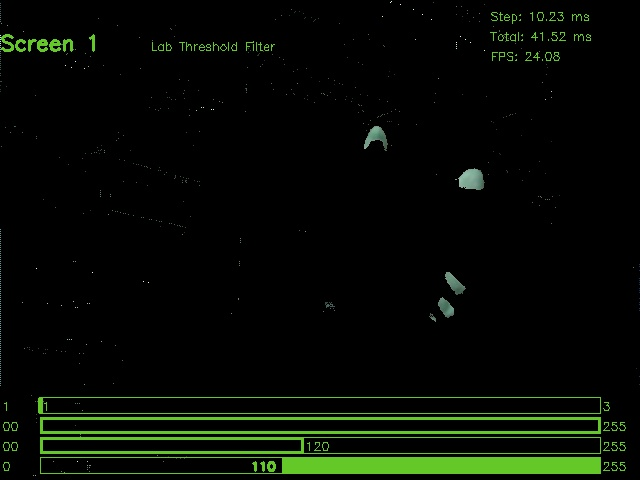
\includegraphics[width=0.23\textwidth]{images/lab_green}}
	\hspace{0.005\textwidth}
	\subfloat[Erosion filter]{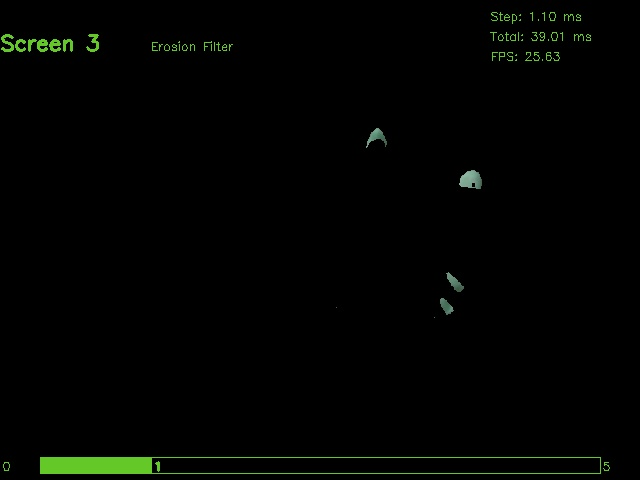
\includegraphics[width=0.23\textwidth]{images/erosion_green}}
	\hspace{0.005\textwidth}
	\subfloat[Lab thresholding filter]{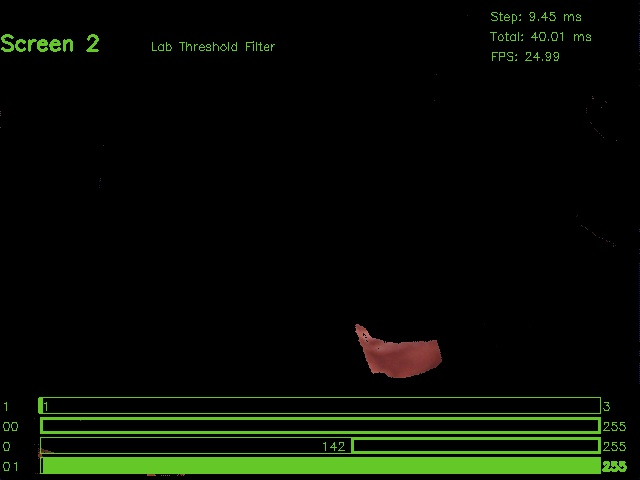
\includegraphics[width=0.23\textwidth]{images/lab_red}}
	\hspace{0.005\textwidth}
	\subfloat[Erosion filter]{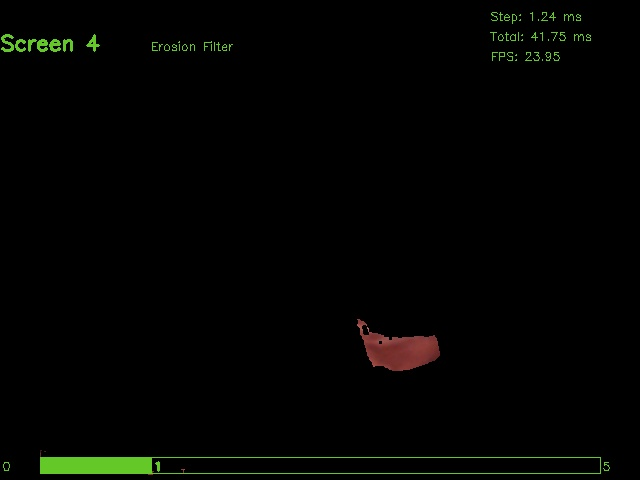
\includegraphics[width=0.23\textwidth]{images/erosion_red}}
	\hspace{0.005\textwidth}
	\subfloat[Blob detection filter]{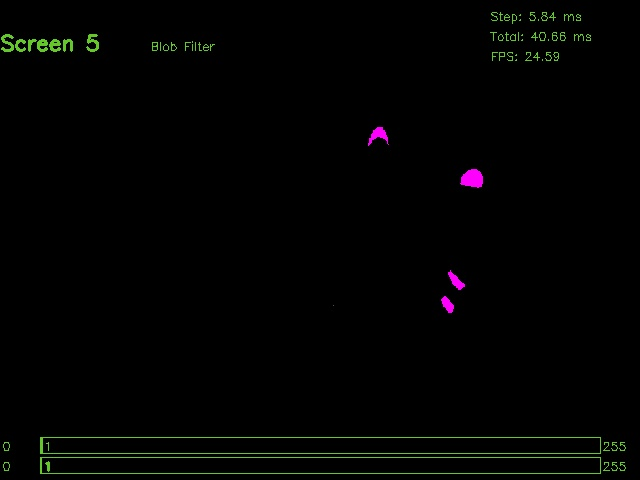
\includegraphics[width=0.23\textwidth]{images/blob_green}}
	\hspace{0.005\textwidth}
	\subfloat[Blob detection filter]{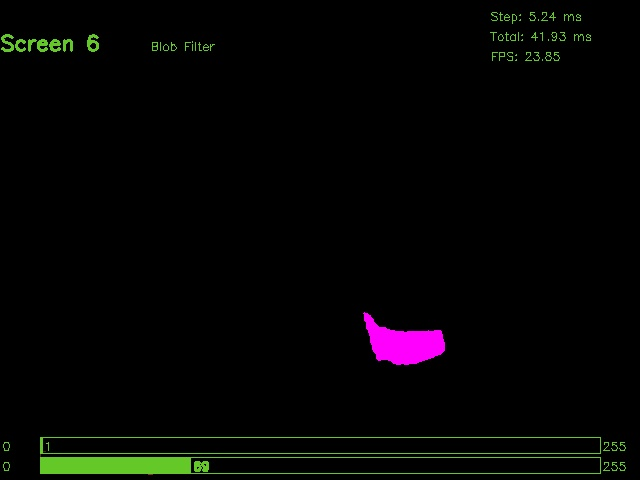
\includegraphics[width=0.23\textwidth]{images/blob_red}}
	\hspace{0.005\textwidth}
	\subfloat[Add filter]{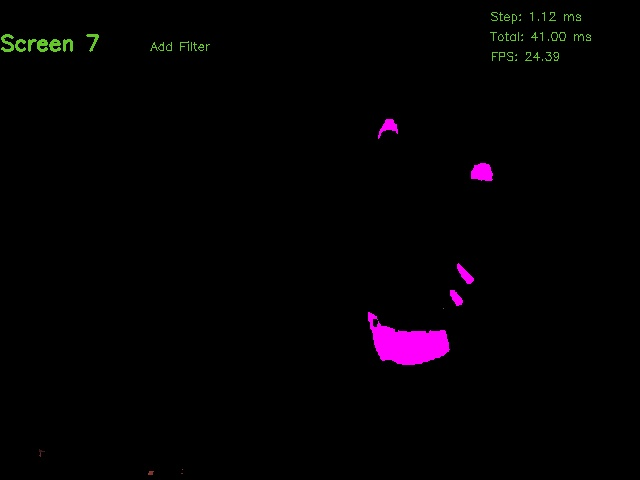
\includegraphics[width=0.23\textwidth]{images/add}}
	\hspace{0.005\textwidth}
	\subfloat[Add filter]{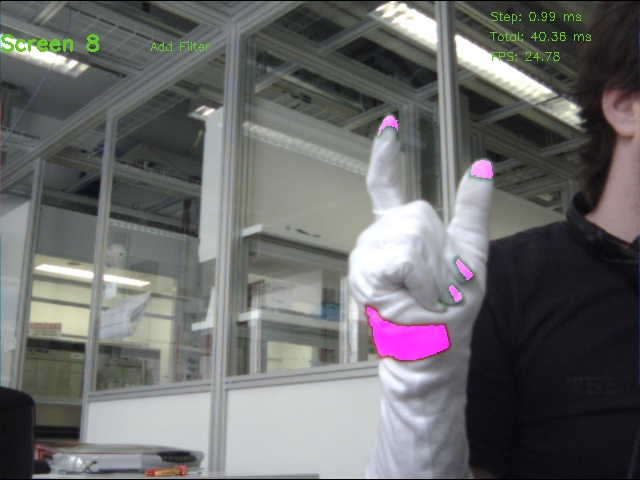
\includegraphics[width=0.23\textwidth]{images/overlay}}
	\caption{Resulting steps from tracker with filter chain from section \ref{sub:chosen-filter-chain}}
	\label{fig:tracker-chain}
\end{figure}


\section{Evaluation results}
\label{sec:evaluation-results}

The different modules and programs have been tested qualitatively with a 55 seconds video recorded at 23 frames per second and containing 23 gestures (5 pointing gestures, 6 zooming gestures and 12 swiping gestures). These 55 seconds of video resulted in 1251 postures and after the sample supervision (see section \ref{sub:sample-supervision})  1219 of them were used for the training (see table \ref{tbl:eval}).

\begin{table}[h]
\caption{Postures and gestures of training video}
\tablestyle
\begin{tabular}{*{3}{v{0.2\textwidth}}}
\toprule
   \tablehead gesture name &
   \tablehead number of gestures & 
   \tablehead number of postures \tabularnewline
\midrule
Nothing & 24 & 317\tabularnewline
Pointing & 5 & 397 \tabularnewline
Zooming & 6 & 253 \tabularnewline
Swiping & 12 & 78 (left) \tabularnewline
 &  & 174 (right) \tabularnewline
\bottomrule
\textbf{Total} & \textbf{47} & \textbf{1219} \tabularnewline
\bottomrule
\end{tabular}
\label{tbl:eval}
\end{table}

Once the trainer has a decision function loaded, either by directly training on a sample library or by loading it from a file, it can directly be tested within the trainer using live images from the camera. Analogue to the display of the label from the subtitle during the sample collection (see section \ref{sub:sample-collection}) the label obtained from the decision function is displayed in the same position, indicating the posture that is currently recognized. The filtered posture (see section \ref{sub:posture-classification}) worked remarkably well as long the setup constraints (see section \ref{sub:environmental-constraints}) and the gesture definitions (see section \ref{sec:gestures}) were respected:

\begin{itemize}
\item the distance between glove and camera during the live test should be similar to this distance in the recorded gestures.
\item the lightning conditions are not extreme: the auto-exposure and the auto-gain of the camera have their limits.
\item no background elements should contain green or red colors.
\item tracker can see the characteristic finger blobs of a posture as well as the wrist blob.
\end{itemize}

However, the posture classification is not working well in the following situations:
\begin{itemize}
\item Sometimes when pointing very low, the red marker can not be detected.
\item Pointing to the far right side, without moving the wrist can be classified as a right posture.
\item During the zooming gesture, when thumb and index fingers almost touch each other the classification can result in a posture that is either classified as the pointing posture or the garbage posture.
\end{itemize}

\section{Use case}
\label{sec:use-case}

For the demonstration of an interface controlled by gestures, a small program was implemented (see figure \ref{fig:demo}). This demo program mapped the three gestures from section \ref{sec:gestures} to the following behaviors:

\begin{itemize}
\item Pointing gesture: moves the cursor
\item Zooming gesture: updates a bar indicating the zoom factor
\item Swiping gesture: lets the interface slide in or out on the right side.
\end{itemize}

\begin{figure}[H]
\center
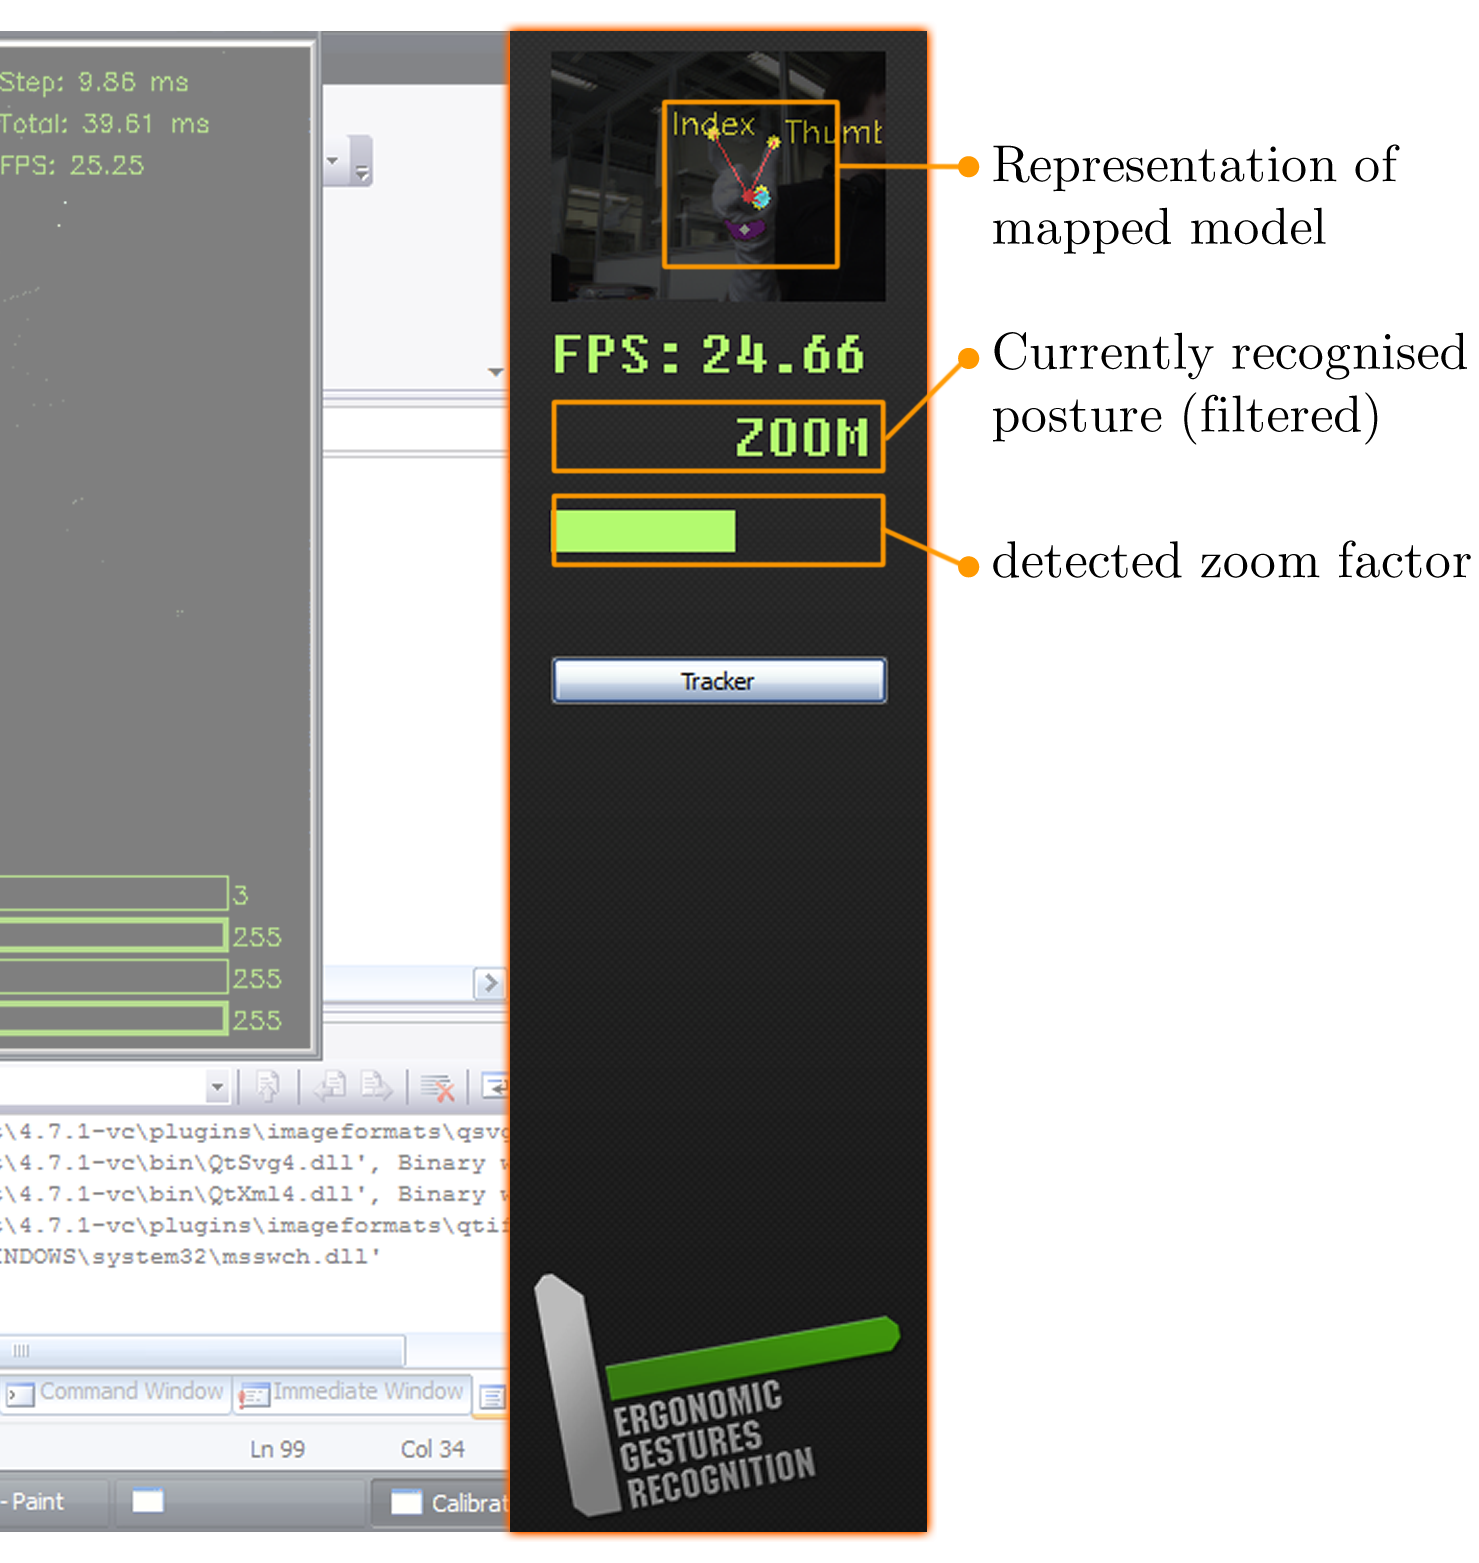
\includegraphics[width=0.7\textwidth]{images/demo} 
\caption{Demo application}
\label{fig:demo}
\end{figure}

This program has no real function other than to demonstrate the recognition of the control gestures. This program was also tested with several other users, who mentioned the following feedback:
\begin{itemize}
\item the reaction time is very fast,
\item the gestures are easy to learn,
\item a real gestural interface would require more gestures, of the same complexity level (i.e. a vertical swipe or grabbing gesture)
\end{itemize}  

